% A listing of the contents of each file supplied as Supporting Information
% should be included. For instructions on what should be included in the
% Supporting Information as well as how to prepare this material for
% publications, refer to the journal's Instructions for Authors.

% The following files are available free of charge.
% \begin{itemize}
% \item Filename: brief description
% \item Filename: brief description
% \end{itemize}

Supplementary figures:
\begin{itemize}
\item \cref{tab:table-mult}
\item \cref{fig:steps-v-corr}
\item \cref{tab:table-versions}
\item \cref{fig:structs-v-corr-id-zemu-12-60000-rscript-validated-t14}
\item \cref{fig:structs-v-corr-WildTypeComplex-ddg-monomer-16-003-zemu-2}
\item \cref{fig:wildtypecomplex-scores-complete}
\item \cref{fig:spear-corr-rmsd-error}
\item \cref{fig:t14-mean-ensemble-error}
\end{itemize}

\subimport*{figs-and-tables/}{table-mult}
\subimport*{figs-and-tables/}{steps-v-corr}
\subimport*{figs-and-tables/}{table-versions}
\subimport*{figs-and-tables/}{structs-v-corr-id-zemu-12-60000-rscript-validated-t14}
\subimport*{figs-and-tables/}{structs-v-corr-WildTypeComplex-ddg-monomer-16-003-zemu-2}

\begin{figure}
  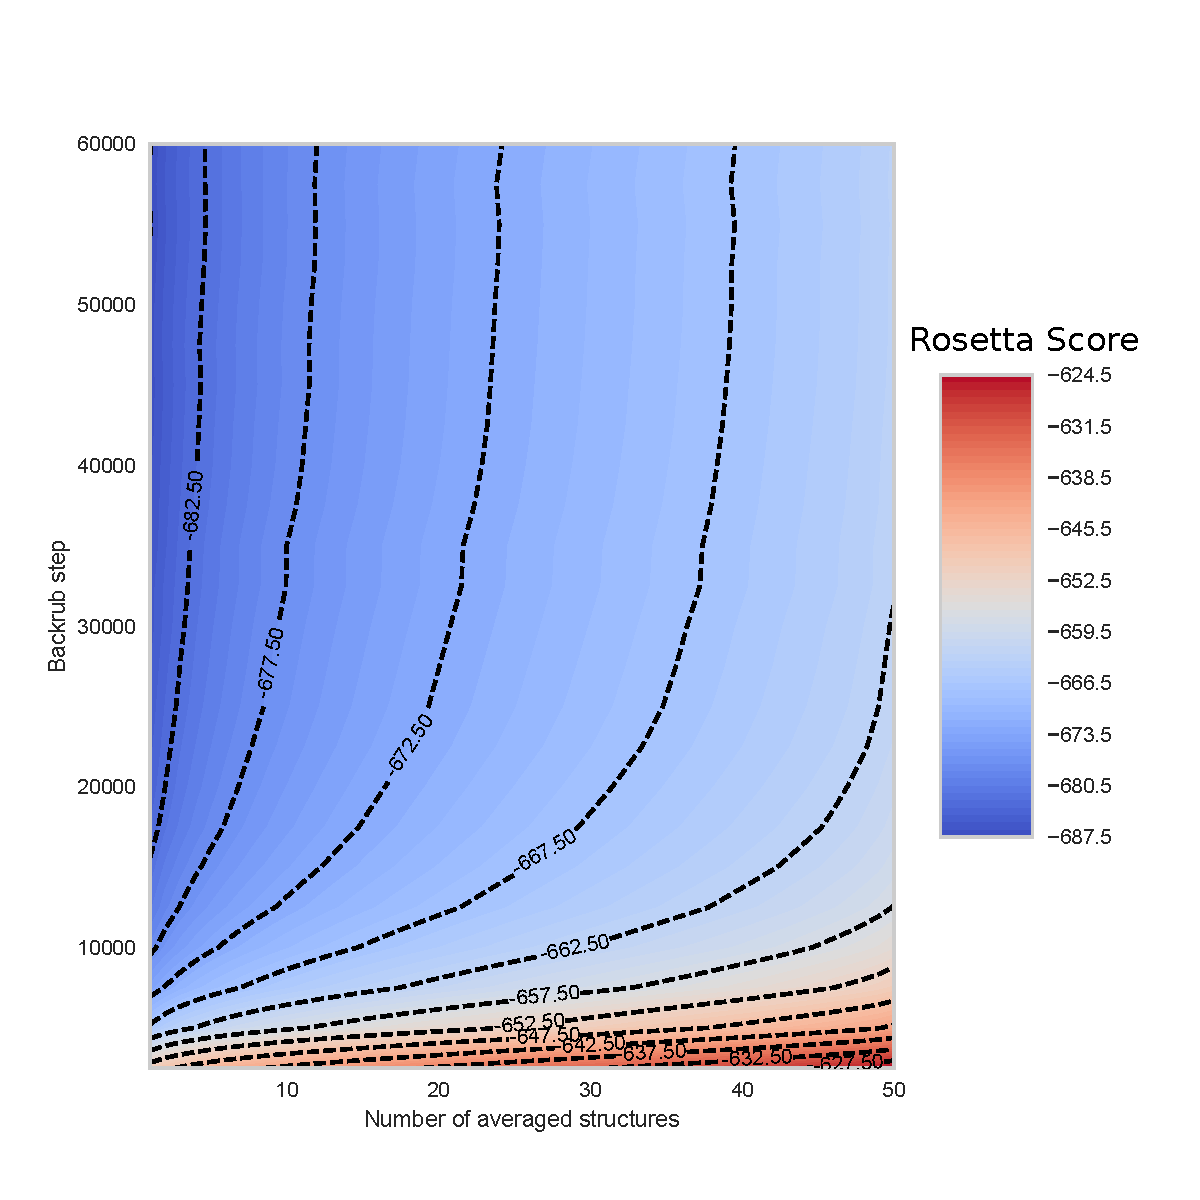
\includegraphics[width=\textwidth,keepaspectratio]{figures/wildtypecomplex-scores-complete.pdf}
  \caption{
    Contour plot showing the effect of backrub sampling on the average wild-type complex score, for varying numbers of averaged models.
  } \label{fig:wildtypecomplex-scores-complete}
\end{figure}

\begin{figure}
  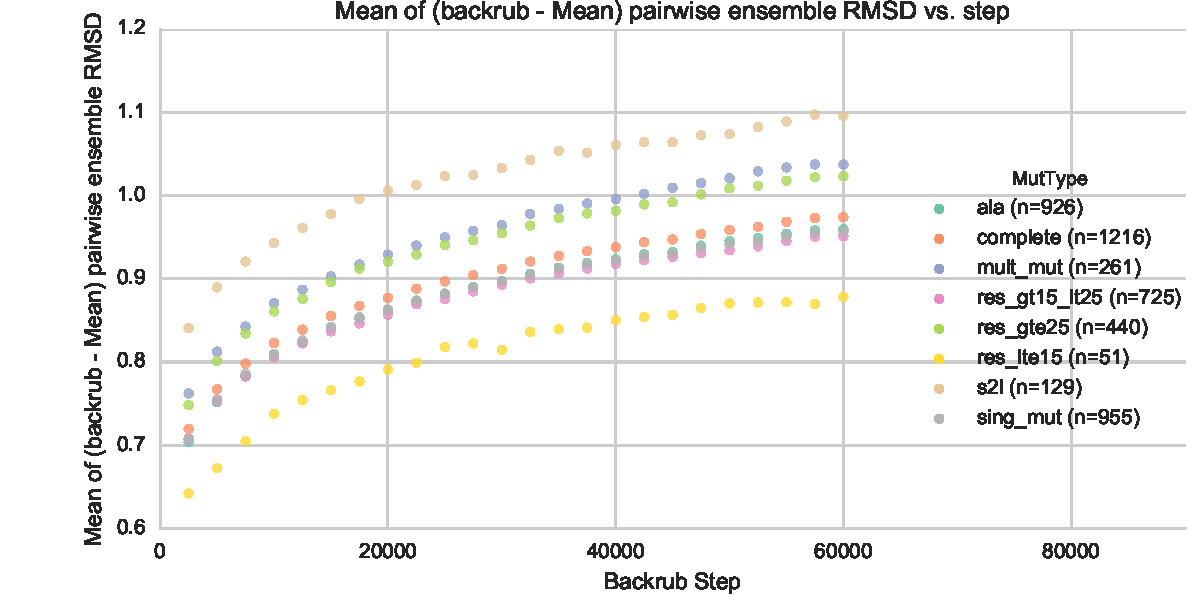
\includegraphics[width=\textwidth,keepaspectratio]{figures/t14-mean-ensemble-error.pdf}
  \caption{
    Mean backrub ensemble RMSD vs. backrub steps.
  } \label{fig:t14-mean-ensemble-error}
\end{figure}

\begin{figure}
  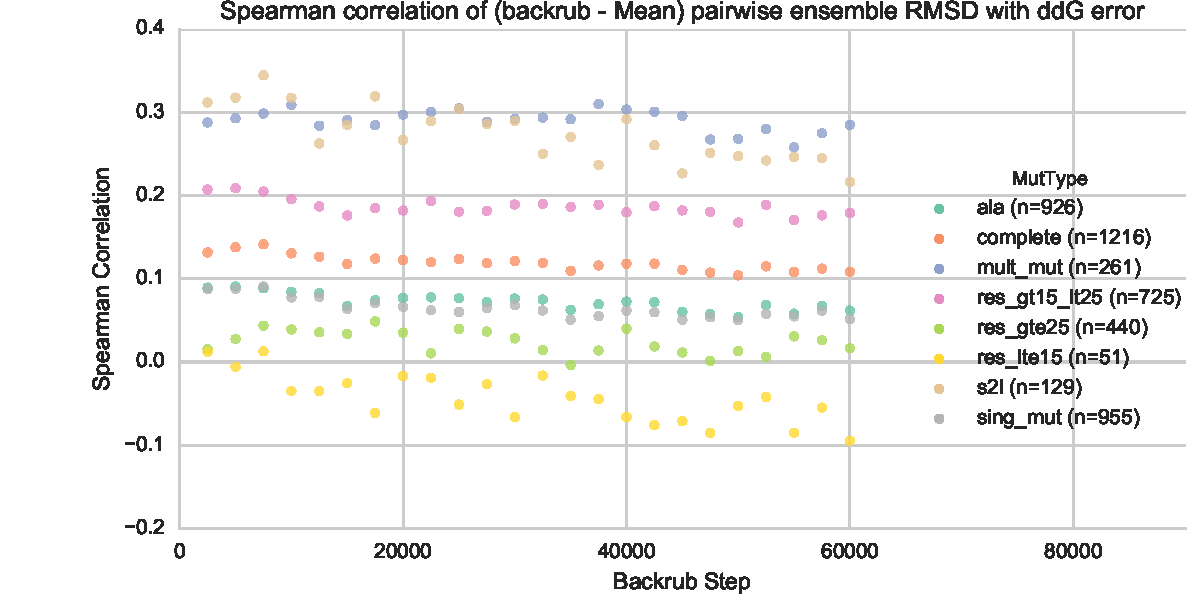
\includegraphics[width=\textwidth,keepaspectratio]{figures/t14-spear-corr.pdf}
  \caption{
    Scatter plot showing the average Spearman correlation of ddG prediction error v. mean backrub ensemble RMSD, v. backrub steps.
  } \label{fig:spear-corr-rmsd-error}
\end{figure}